% !TeX spellcheck = en_US
\documentclass[french]{yLectureNote}

\title{Électromagnétisme 1 PS}
\subtitle{Physique}
\author{Paulhenry Saux}
\date{\today}
\yLanguage{Français}
%lionels.calmels@cemes.fr
\professor{F.Pettinari}
\usepackage{graphicx}%----pour mettre des images
\usepackage[utf8]{inputenc}%---encodage
\usepackage{geometry}%---pour modifier les tailles et mettre a4paper
%\usepackage{awesomebox}%---pour les boites d'exercices, de pbq et de croquis ---d\'esactiv\'e pour les TP de PC
\usepackage{tikz}%---pour deiffner + d\'ependance de chemfig
% \usepackage{tabularx}%---pour dimensionner automatiquement les tableaux avec variable X
\usepackage{awesomebox}%---Pour les boites info, danger et autres
\usepackage{menukeys}%---Pour deiffner les touches de Calculatrice
\usepackage{fancyhdr}%---pour les en-t\^ete personnalis\'ees
\usepackage{blindtext}%---pour les liens
\usepackage{hyperref}%---pour les liens (\`a mettre en dernier)
\usepackage{caption}%---pour la francisation de la l\'egende table vers Tableau
\usepackage{pifont}
\usepackage{array}%---pour les tableaux
\usepackage{lipsum}
\usepackage{yFlatTable}
\usepackage{multicol}
\newcommand{\Lim}[1]{\lim\limits_{\substack{#1}}\:}
\renewcommand{\vec}{\overrightarrow}
\newcommand{\N}[0]{\mathbb{N}}
\newcommand{\dd}{\mathrm{d}}
\newcommand{\norm}[1]{||\vec{#1}||}
\newcommand{\fo}{\psi(\vec{r},t)}
\newcommand{\foe}{\psi(\vec{r},t)\*}
\newcommand{\HH}{\hat{H}}
\newcommand{\hb}{\hbar}
\newcommand{\lap}{\nabla^2}
\newcommand{\lapcc}{\frac{\partial^2 }{\partial x^2}+\frac{\partial^2 }{\partial y^2}+\frac{\partial^2 }{\partial z^2}}
\newcommand{\E}{\vec{E}(M)}
\newcommand{\V}{V(M)}
\newcommand{\er}{\vec{e_{\rho}}}
\newcommand{\ep}{\vec{e_{\varphi}}}
\newcommand{\pip}{\pi^+}
\newcommand{\pim}{\pi^-}
\begin{document}
\setcounter{chapter}{2}
\chapter{Généralité sur le champ et potentiel}
\section{Propriété de symétrie}
\subsection{Pour un point dans un plan \(\pi^+\)}
On prend comme exemple M contenu dans le plan médiateur de 2 charges ponctuelles.
%TODO s1 schema


\includegraphics[scale=0.5]{s1}

On a \(\vec{E_2(M)} = \frac{q_2}{4\pi\epsilon_0 \norm{P_2M}}\vec{e_{P_2M}}\) et \(\vec{E_1(M)} = \frac{q_1}{4\pi\epsilon_0 \norm{P_1M}}\vec{e_{P_1M}}\)

Mais comme \(\norm{P_1M} = \norm{P_2M}\) et \(q_1=q_2\), on a \(\norm{E_1(M)} = \norm{E_2(M)}\)

On en déduit que si \(M\in \pi^+, \E\)\marginCritical{Le fait que M doivent appartenir au plan est primordial} est contenu dans ce plan qui passe par M.

\warningInfo{Remarque}{Si \(M\in\) plusieurs plans, alors \(\E\) est contenu dans leur intersection (si\(\E\neq \vec{0}\)).}
\subsection{Pour un poinr dans un plan \(\pi^-\)}

\includegraphics[scale=0.5]{s2}

On a de la m\^eme façon \(\norm{P_1M} = \norm{P_2M}\) et \(|q_1|=|q_2|\) donc \(\norm{E_1(M)} = \norm{E_2(M)}\)

On en déduit que \(\E\) est orthogonal au plan \(\pi^-\).
\subsection{Plans \(\pi\) ne passant pas par M}
Dans ce cas, l'existence de ces plans ne donnent aucune information sur la direction du vecteur \(\E\) !
\subsection{Vecteurs vrais/polaire}
On dit que les vecteurs possédants les \^emes propriétés que \(\E\), i.e. \(\E \in \pi^+, \E \perp \pi^-\) passant par M sont dit vrais. Ce qui relie le point M à la source ne fait pas intervenir le produit vectoriel.
\section{Propriétés d'invariance}
\begin{theorem}[Principe de Curie]
 Les effets ont au moins les symétries de leur cause
\end{theorem}
Ici, les effets sont \(\E, \V\) et les causes la distribution de charge.

Donc si cette dernière possède des invariances, les composantes non  nulle de \(\E\) dans la base judicieusement choisie et \V possèdent les m\^emes invariances.
\section{Propriété de parité de \(\E, \V\) autour de plans}
\subsubsection{Plan +}

\includegraphics[scale=0.5]{s3}

On remarque que \(\norm{E_1(M_1)} = \norm{E_2(M)}\) et \(\norm{E_2(M_1)} = \norm{E_1(M)}\) mais aussi que \(\norm{E_1(M)}>\norm{E_2(M)}\)

On en déduit que \(E_x(x,y,z) = E_x(x,y,-z)\), \(E_y(x,y,z) = E_y(x,y,-z)\) et \(E_z(x,y,z) =- E_z(x,y,-z)\).
\subsubsection{Plan -}
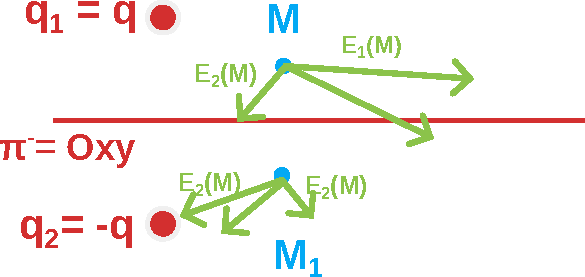
\includegraphics[scale=0.5]{s4}

On remarque que \(E_x(x,y,z) = - E_x(x,y,-z)\), \(E_y(x,y,z) = - E_y(x,y,-z)\) et \(E_z(x,y,z) = E_z(x,y,-z)\).
% \section{Exemples}
% \subsection{\(\E\) crée par un plan infini}
% 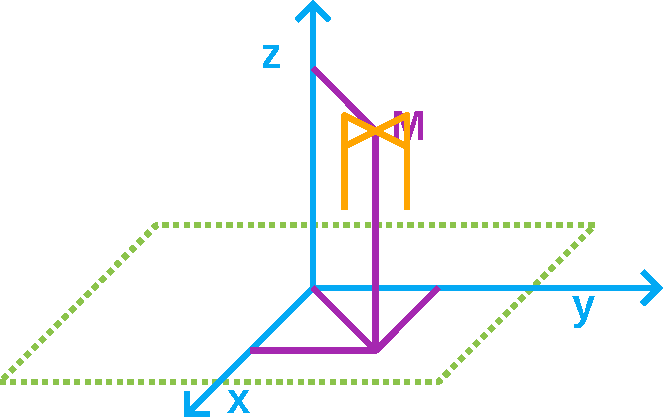
\includegraphics[scale=0.5]{s5}
% \subsubsection{Système de coordonnées}
% Ce système n'est ni à symétrie sphérique ou circulaire\marginCritical{C'est pas cylindrique car il n'y a pas un UNIQUE axe de rotation}, on prend donc des coordonnées cartésiennes pour repérer \(M\) et on utlise la base cartésienne locale \(B(\vec{e_x}, \vec{e_y},\vec{e_z})\).
%
% On place l'origine sur le plan chargé pour tirer partie des propriétés de parité et on prend \(\vec{e_z}\perp \) au plan
% \subsubsection{Symétries}
% Tous les plans verticaux passant par M sont des \(\pi^+\) passant par M. \(\E\) étant un vecteur vrai (\(\in \pi^+\)) passant par M (intersection), \(\E \in axe(M, \vec{e_z})\) et \(\E = E_z(x,y,z)\vec{e_z}\)
% \subsubsection{Invariance}
% Le système est invariant par translaation\marginCheck{Comme il n'y a pas de symétrie circulaire, on envisage pas des symétries par rotation (m\^eme si il peut y en avoir)} selon \(\vec{e_x}, \vec{e_y}\).
%
% Par le principe de Curie, \(E_z(x,y,z)\vec{e_z}\) ne dépend que de z : \(E_z(z)\vec{e_z}\)
% \subsubsection{Parité / Imparité}
% Le plan chargé est un plan \(\pi^+\), donc \(E_z(-z) = - E_z(z)\) qui est impaire de z. De plus, \(V(z)  = V(-z)\) qui est paire de z.
% \subsubsection{Bilan}
% On sait que \(\E = E_z(z), E_z(-z) = - E_z(z), V(-z)  =V(z)\)
% \subsection{Cylindre infiniment long chargé en volume}
% \subsubsection{Base + Coordonnées}
% 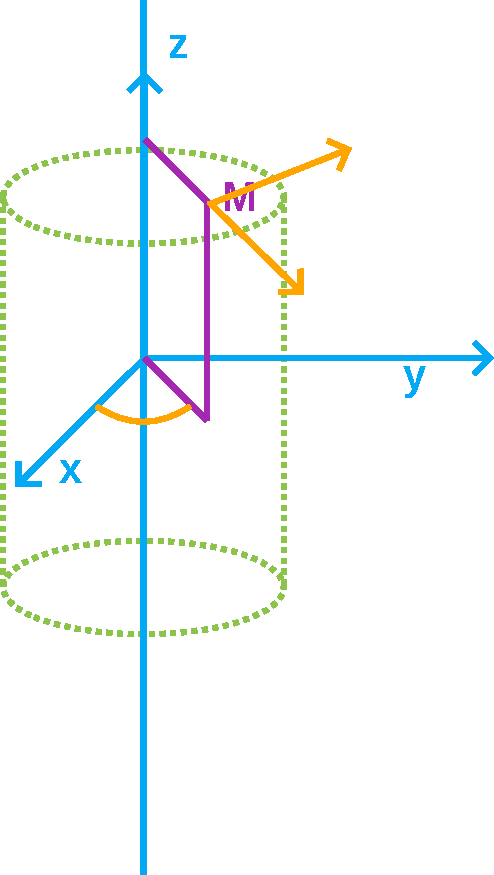
\includegraphics[scale=0.5]{s7-1}
%
% La distribution de charge est à symétrie cylindrique autour de l'axe (Oz) du cylindre chargée, donc on va utiliser la base cylindrique locale \(\vec{e_{\rho}}, \vec{e_{\varphi}}, \vec{e_z}\)
% \subsubsection{Symétries}
% 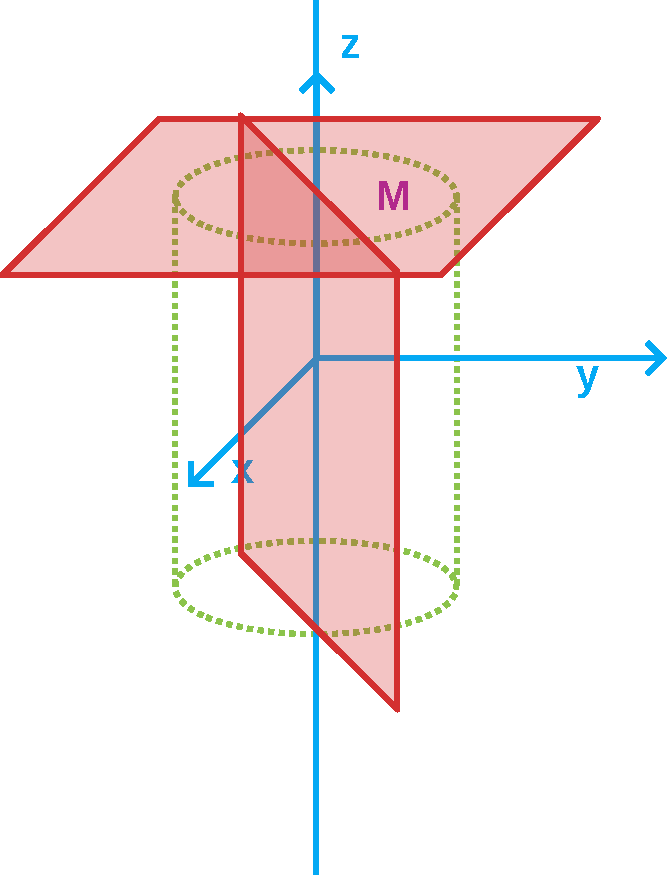
\includegraphics[scale=0.5]{s7-2}
%
% On remarque que \(M, \vec{e_{\rho}}, \vec{e_{\varphi}}\) et \(M, \vec{e_{\rho}}, \vec{e_{z}}\) sont des plans \(\pi^+\) passant par M
%
% On en déduit que \(\E\) est vrai et qu'il appartient aux 2 plans ci-dessus. Donc il est parralèle à l'axe \(\vec{e_{\rho}}\) et \(\E = E_{\rho}(\rho, \varphi, z)\vec{e_{\rho}}\)
% \subsubsection{Invariances}
% Le système (Cylindre  + Point) est invariant par
% \begin{itemize}
%  \item rotation (\(\varphi\)) du cylindre autour de Oz
%  \item translation du cylindre le long de Oz
% \end{itemize}
% On en déduit que \( E_{\rho}(\rho, \varphi, z)\vec{e_{\rho}} =  E_{\rho}(\rho)\vec{e_{\rho}}\) et \(V(M) = V(\rho)\).
% \subsection{Cylindre de longueur L chargé en surface }
% 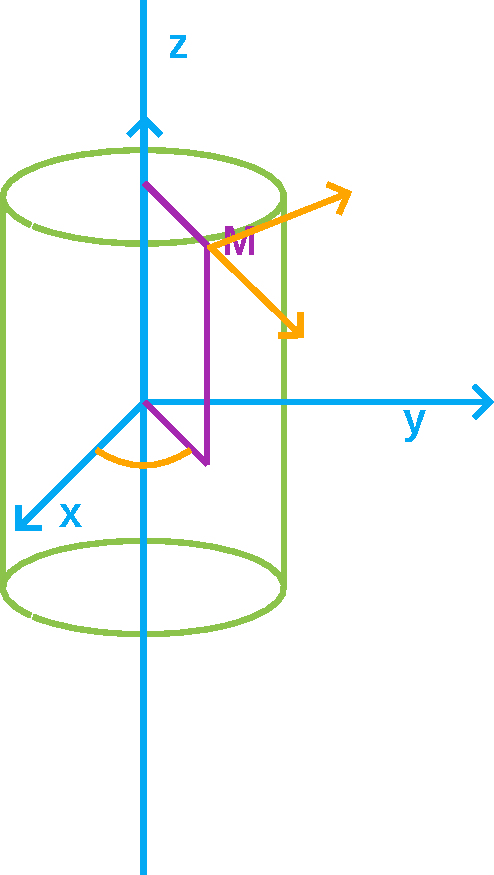
\includegraphics[scale=0.5]{s8-1}
%
% La distribution de charge est à symétrie cylindrique autour de l'axe (Oz) du cylindre chargée, donc on va utiliser la base cylindrique locale \(\vec{e_{\rho}}, \vec{e_{\varphi}}, \vec{e_z}\)
%
% On choisit l'origine au centre du cylindre pour mieux utiliser les propriétés de symétrie.
%
% Le seul \(\pi^+\) est \(M, \vec{e_{\rho}}, \vec{e_{z}}\), donc \(\E\) est vrai à ce \(\pi^+\) et \(\E = E_{\rho}\vec{e_{\rho}} + E_{z}\vec{e_{z}}\)
%
% 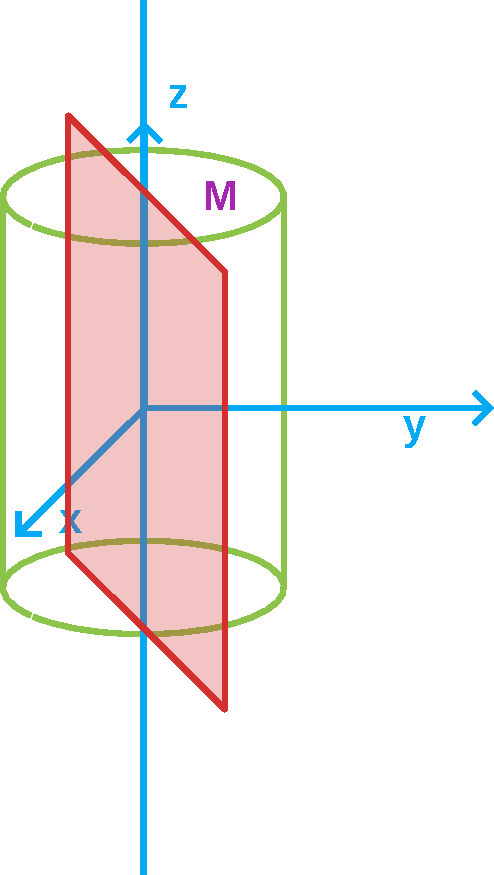
\includegraphics[scale=0.5]{s8-2}
%
% \subsubsection{\(M\in (Oxy)\)}
% On peut retrouver le plan \(M, \vec{e_{\rho}}, \vec{e_{\varphi}}\) et on retrouve le résultat du cylindre infini.
% \subsubsection{\(M\in (Oz)\)}
% Tous les plans contenant (Oz) sont \(\pi^+\), et \(\E\) appartient à leur intersection et \(\E = E_z\vec{e_z}\)
% \subsubsection{Si M est à l'origine}
% Tous les plans contenant Oz et le plan (Oxy) sont \(\pi^+\). Si \(\E\neq 0\), il doit appartenit à chacun de ces plans, ce qui est impossble donc \(\E = \vec{0}\)
% \subsubsection{Invariances quand M quelconque}
% Le sytème n'est invariant que par rotation \(\varphi\) autour de Oz, donc \(\E = E_{\rho}\vec{e_{\rho}} + E_{z}\vec{e_{z}}\) ne dépend pas de \(\varphi\).
%
% Donc \(\E = E_{\rho}(\rho, z)\vec{e_{\rho}} + E_{z}(\rho, z)\vec{e_{z}}\)
% \subsection{Une sphère chargée en volume}
% 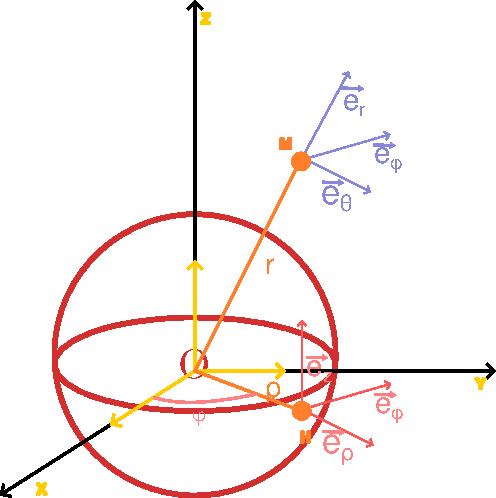
\includegraphics[scale=0.5]{s9}
% La distribution de charge est à symétrie sphérique autour du centre de la sphère. Donc on chosit les coordonnées sphériques et on choisit O le centre de la sphère, avec une base sphérique.
%
% On cherche maintenant les symétries :
%
% Tout plan contenant l'axe (OM) est un plan \(\pip\) passant par M. Il y en a une infinité.
%
% De plus, \(\E\) est vrai et appartient à leur intersection. On en déduit qu'il n'y a qu'une composante nulle : \(E_r(M)\vec{e_r}\)
%
% Étudions les invariances : Le système est invariant par toute rotation par n'importe quel angle autour du point O, en particulier par rotation de la sphère de \(\Delta \varphi\) autour de \((O_z)\) et de \(\Delta \theta\) outour de \(0,\ep\).
%
% Par le principe de Curie, \(E_r(M) = E_r(r), V(M)=V(r)\)
%
% \warningInfo{Remarque}{On cherche la valeur de \(E(0)\) qui appartien à tous les plans \(\pip\) passant par O. Il y en a une infinité, donc c'est impossible.}
\section{Lien entre \(\E\) et \(\V\)}
\subsection{Équation intégrale entre E et V}
\begin{theorem}[Équation intégrale]
\[V(B)-V(A) = -\int_A^B\E\cdot \dd \vec{l}(M)\]
\end{theorem}
Si \(B\to A\), l'intégrale est nulle et \(V(B\to A) = V(A)\) donc V est une fonction continue des coordonnées de M.

\subsection{Équation locale entre E et V}
\begin{theorem}[Équation locale entre E et V]
\[\dd V = -\E\cdot \dd \vec{l}(M)\]
\[\E = -grad(\V)\]
\end{theorem}
% On a \(V(M') = V(M)+\dd V(M)\), i.e. si on passe de M à M', alors le potentiel  varie comme indiqué.
%
% Ainsi, dans la BOND cartésienne, on a \(\dd (V) = -E_x \dd x - E_y \dd y - E_z \dd z\). On peut aussi écrire \(\dd V = \frac{\partial V(x,y,z)}{\partial x}\dd x + \dots + \frac{\partial V(x,y,z)}{\partial z}\dd z\).
%
% On déduit de ces 2 équations : \(E_x - \frac{\partial V(x,y,z)}{\partial x}, \dots, E_z - \frac{\partial V(x,y,z)}{\partial z}\).
%
% On en déduit la seconde forme de l'EQL :
\criticalInfo{Gradient dans les 3 systèmes de coordonnées (À savoir)}{
\[grad\:g(\rho, \varphi, z) = \frac{\partial g}{\partial \rho}, \frac{1}{\rho} \frac{\partial g}{\partial \varphi}, \frac{\partial g}{\partial z} \]

\[grad\: h(r,\theta,\varphi) = \frac{\partial h}{\partial r}, \frac{1}{r}\frac{\partial h}{\partial \theta}, \frac{1}{r\sin(\theta)}\frac{\partial h}{\partial \varphi}\]

On remarque que le dénominteur correspond au déplacement élémentaire
}
\section{Lignes de champ électrique}

\includegraphics[scale=0.5]{s10}
\begin{definition}[Ligne de champ]
Les lignes du champ électrique sont l'ensemble des courbes en tout point desquel le champ électrique à la ligne de champ. Elles sont orientées de la sens du champ électrique.
\end{definition}
% Tracer les lignes de champ permet de cartographier le champ dans l'espace.
%
% Exemple de 2 particules dans l'espace
% %TODO s11 (à améliorer )
\section{Surfaces équipotentielles}
\begin{definition}[Surface équipotentielle]
La surface équipotentielle de potentiel \(V_0\) est l'ensemble des points M tel que \(\V = V_0\)
\end{definition}
2 surfaces distinctes ne se coupent jamais.

% Exemple des 2 particules de charge contraire :
%
% %TODO Schema à faire

\section{Lien entre surfaces equipotentielles et lignes de champ}

\begin{theorem}[Ligne de champ et Surface équipotentielle]
Les lignes de champ sont perpendiculaires aux surfaces de champ qu'elles coupent.
\end{theorem}
% \begin{myproof}
%  On considère 2 points infiniment proches : \(\dd l = \vec{MM'}\) et \(V(M') = V(M)+\dd V(M)\). De plus,  \(\dd V = -\E \cdot \dd \vec{l}\).
%
% Si \(M, M'\) appartiennent à la m\^eme surface équipotentielle, \(V(M) = V(M') \Rightarrow \dd V(M) = 0\). On en déduit que \(\E\cdot \dd \vec{l} = 0\), et comme \(\E \neq \vec{0}), \E \perp \dd \vec{l}\).
% \end{myproof}

\begin{theorem}[Orientation des lignes de champ]
 Les lignes de champ sont orienté dans le sens des potentiels décroissants.
\end{theorem}
% \begin{myproof}
%  On considère \(M_1\) sur la surface \(V_2\) et \(M_2\) sur \(V_2\). On suppose que les 2 points sont liés par la m\^eme ligné de champ.
%
% On suppose de plus que M est un point quelconque sur la ligne de champ entre \(M_1\) et \(M_2\) et que \(\E\) est orienté de \(M_1\) vers \(M_2\).
%
% On applique l'équation intégrale entre E et V :
% \begin{equation*}
% V(M_2)-V(M_1) = -\int_{M_1}^{M_2}\E\cdot \dd \vec{l}(M)
% \end{equation*}
% On en déduit que \(\dd \vec{l}\) est orienté de \(M_1\) vers \(M_2\).
%
% Avec ces hypothèses, on déduit que l'intégrale est sytictement positive, donc que \(V(M_2)-V(M_1) <0 \Rightarrow V(M_2)<V(M_1)\)
% \end{myproof}

 \end{document}
